\section{KẾT QUẢ}\label{sec:ket-qua}
\hspace{1cm}

Môi trường demo được khởi tạo theo một trong hai cách: chạy
\texttt{bash scripts/seed\_db.sh} (tạo schema, Extract, Transform,
Load rồi chạy kiểm tra chất lượng, sau đó train mô hình trong container bằng
\texttt{POST /risk/retrain}), hoặc kích hoạt DAG \texttt{staging\_load} trên Airflow để
chuỗi \texttt{staging\_load} $\to$ \texttt{dw\_load} $\to$ \texttt{dss\_batch} tự chạy. 
% Các
% dịch vụ backend khởi động bằng \texttt{docker compose up -d}, với Airflow UI tại cổng 8080,
% DSS service tại cổng 8001, backend API tại cổng 8000 và PostgreSQL tại cổng 5433; frontend
% chạy riêng bằng \texttt{npm run dev} tại cổng 5173.

\textbf{Kết quả:} Kích hoạt \texttt{staging\_load} trên Airflow, cả ba DAG chạy thành
công nối tiếp nhau, mỗi DAG dưới một phút. Chạy lại không làm thay đổi số dòng (98.666 đơn trong
\texttt{FACT\_ORDER\_FULFILLMENT}, 96.355 phiên bản khách hàng, 38.229 điểm rủi ro) và chỉ số
mô hình giữ nguyên, xác nhận pipeline idempotent và kết quả lặp lại được.

% \textbf{Lưu ý về phiên bản thư viện.} File mô hình (\texttt{dss/models/*.pkl}) phải được huấn
% luyện bằng cùng phiên bản scikit-learn với container \texttt{dss} (1.9.1); mô hình train trên
% máy với phiên bản khác không nạp được trong container. Vì vậy mô hình luôn được huấn luyện lại
% bên trong container qua \texttt{POST /risk/retrain} (DAG \texttt{dss\_batch}).


% \textbf{Tài liệu trình bày và tái lập kết quả.}
% \begin{itemize}
%     \item \texttt{dss/notebooks/\allowbreak risk\_models.ipynb}: notebook đi lại từng bước của
%           \texttt{dss/risk/\allowbreak train.py} -- đọc dữ liệu từ kho, khám phá dữ liệu, đặc trưng và chống
%           leakage, chia theo thời gian, huấn luyện HGB và baseline, ngưỡng theo chi phí, đường
%           precision--recall, feature importance, thí nghiệm chấm điểm sớm và drift, what-if. Notebook
%           gọi chính các hàm của project và chỉ đọc kho dữ liệu, nên số liệu khớp với hệ thống
%           và với Chương~6.
%     \item \texttt{report/scripts/make\_figures.py}: vẽ lại các biểu đồ của Chương~6 (tỷ lệ trễ
%           theo tháng, đường precision--recall, feature importance) trực tiếp từ kho dữ liệu sau
%           mỗi lần huấn luyện lại.
% \end{itemize}


Frontend gồm bốn màn hình chọn qua thanh tab: 
\begin{itemize}
      \item \textbf{Manager Dashboard} (KPI, doanh thu theo tháng và theo bang có bộ lọc năm/ngành/vùng, giao hàng và mức độ hài lòng, sản phẩm doanh thu cao nhất/thấp nhất)
      \item \textbf{Ops Console} (đơn có rủi ro giao trễ hoặc đánh giá thấp, \textit{Simulate action} mô phỏng kéo dài ngày hẹn giao, gắn khách vào chiến dịch)
      \item \textbf{Campaign} (quản lý chiến dịch và khách đã gắn)
      \item \textbf{Risk Predictor} (chấm điểm rủi ro cho một đơn tự nhập, Mục~\ref{sec:dss-whatif})
\end{itemize}
Các danh sách đều cho phép chọn số dòng và tải về tệp \texttt{.csv}/\texttt{.xlsx}.

Hình~\ref{fig:ui-manager}--\ref{fig:ui-predict} là ảnh chụp bốn màn hình khi chạy với dữ liệu thật.

\begin{figure}[H]
\centering
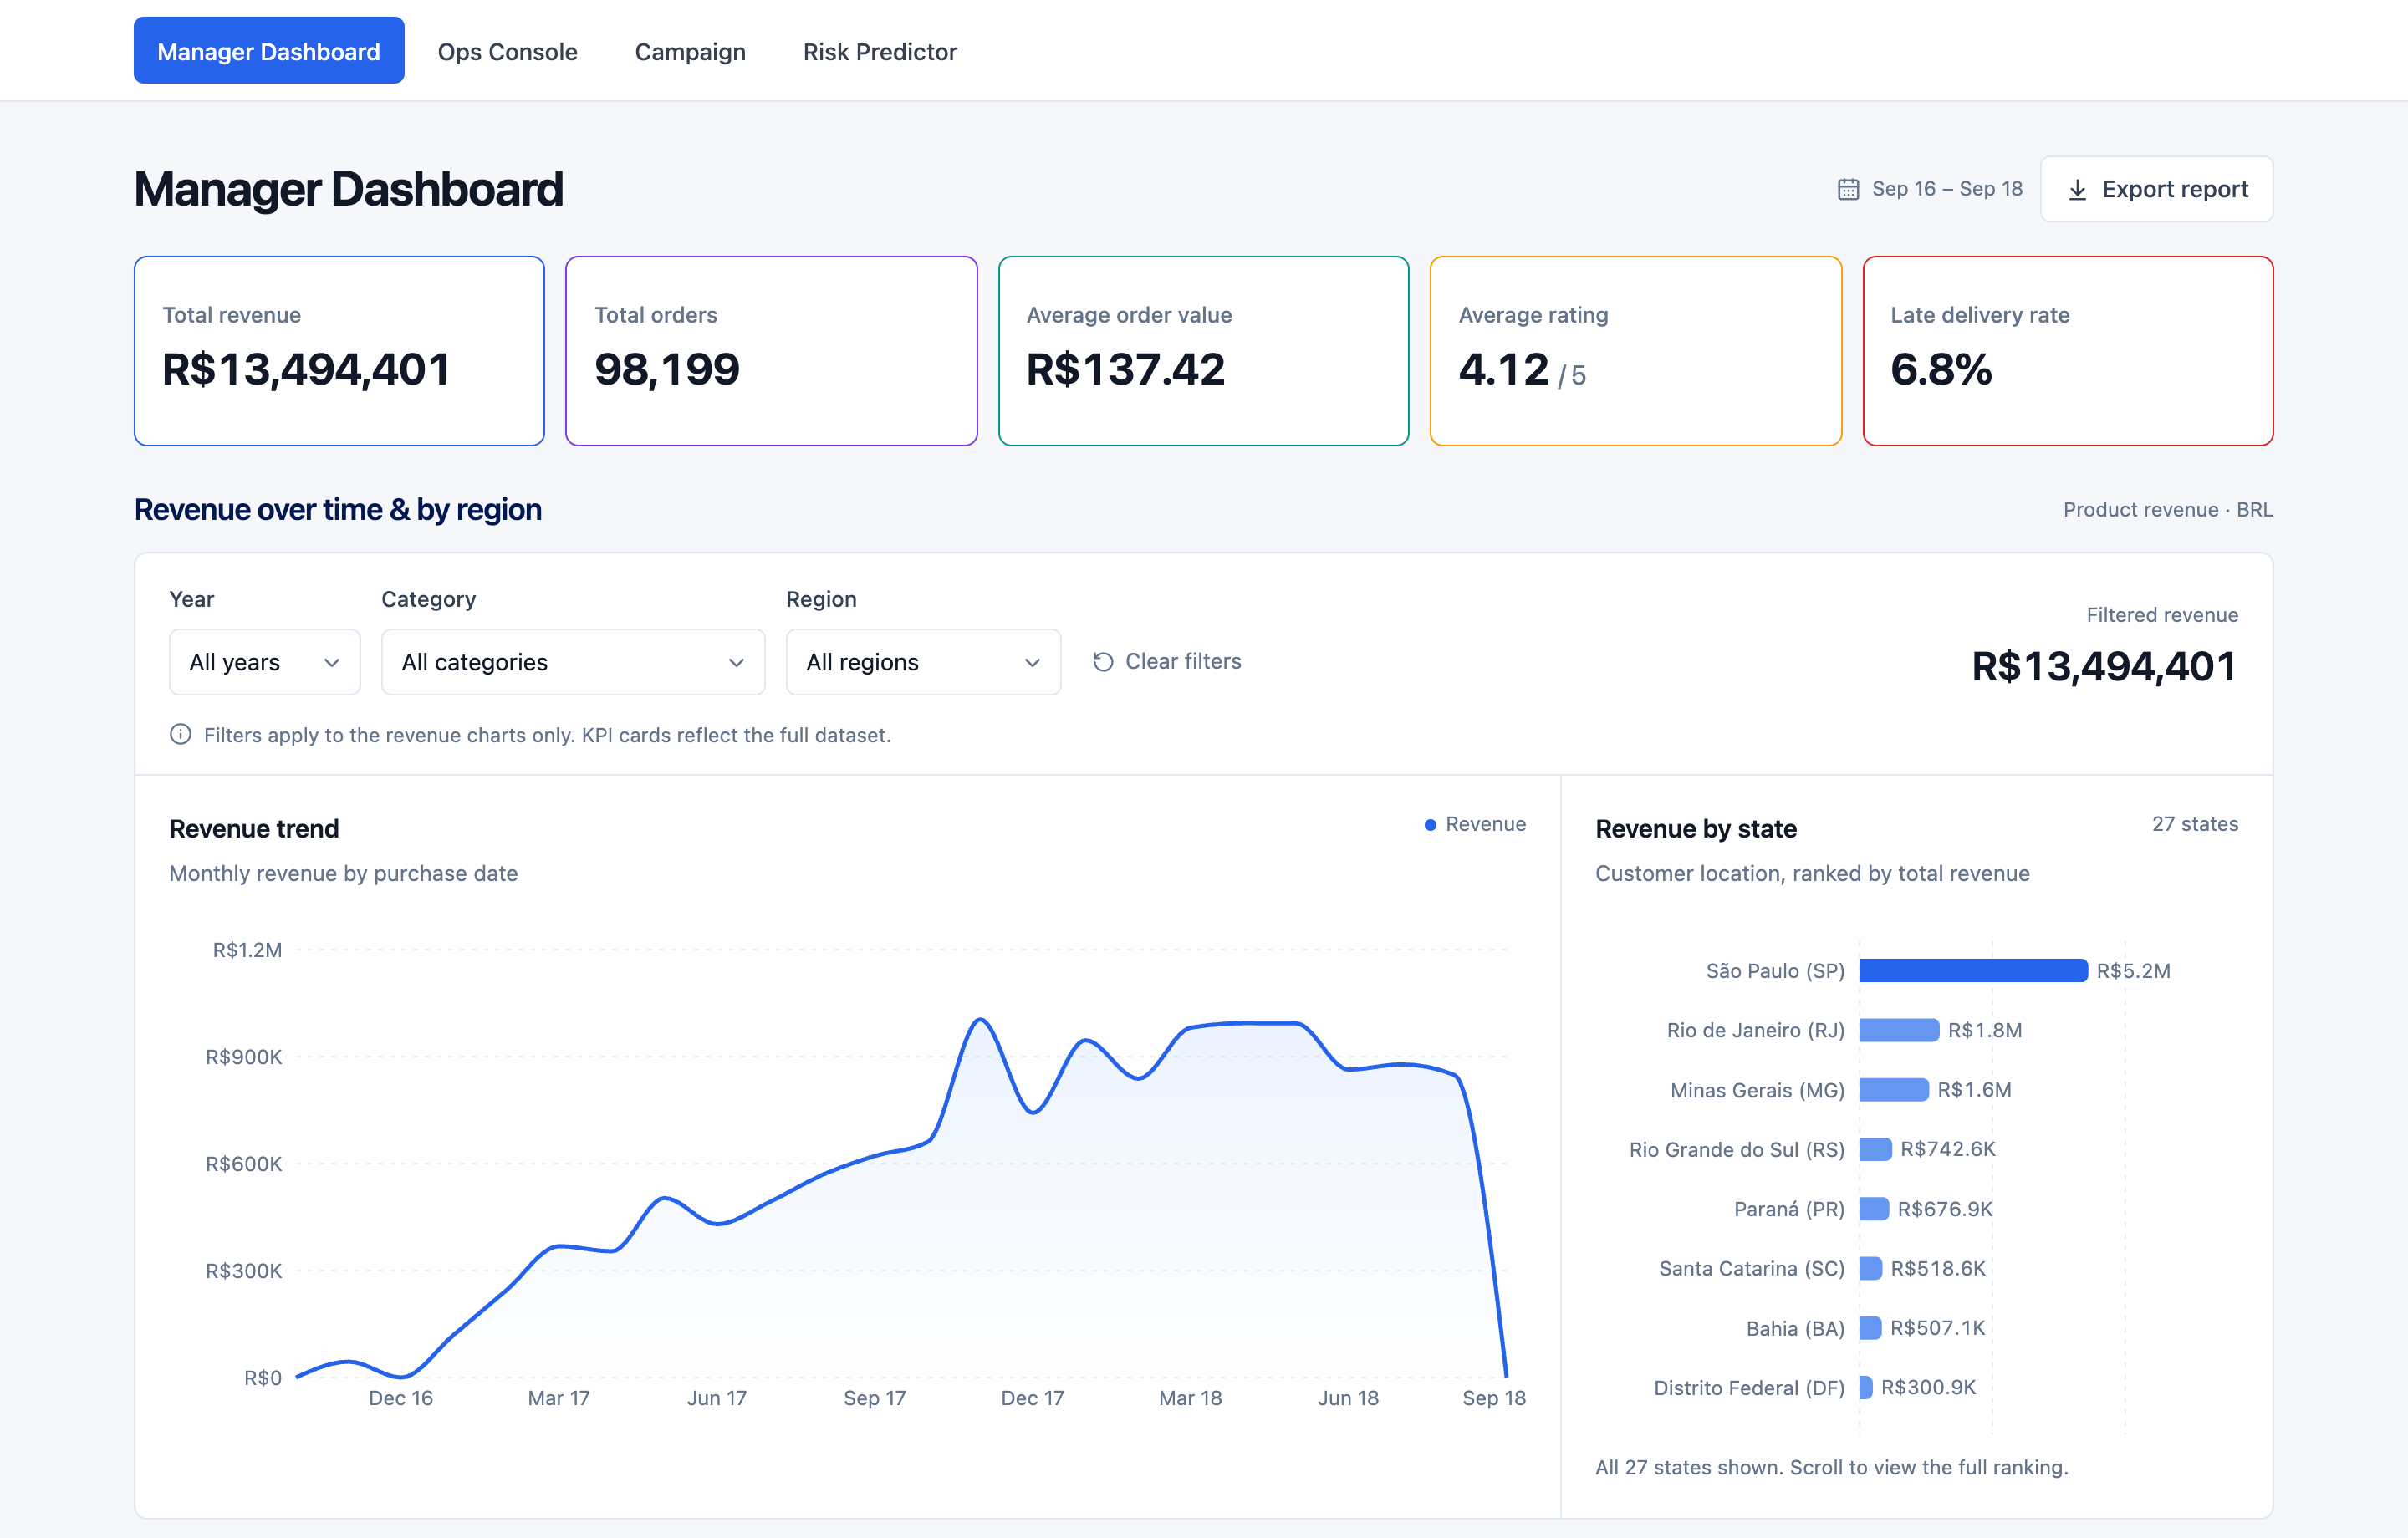
\includegraphics[width=0.75\textwidth]{Picture/ui_manager_overview.png}
\caption{Manager Dashboard: thanh tab trên cùng, thẻ KPI, doanh thu theo tháng và theo bang với bộ lọc năm/ngành/vùng}
\label{fig:ui-manager}
\end{figure}

\begin{figure}[H]
\centering
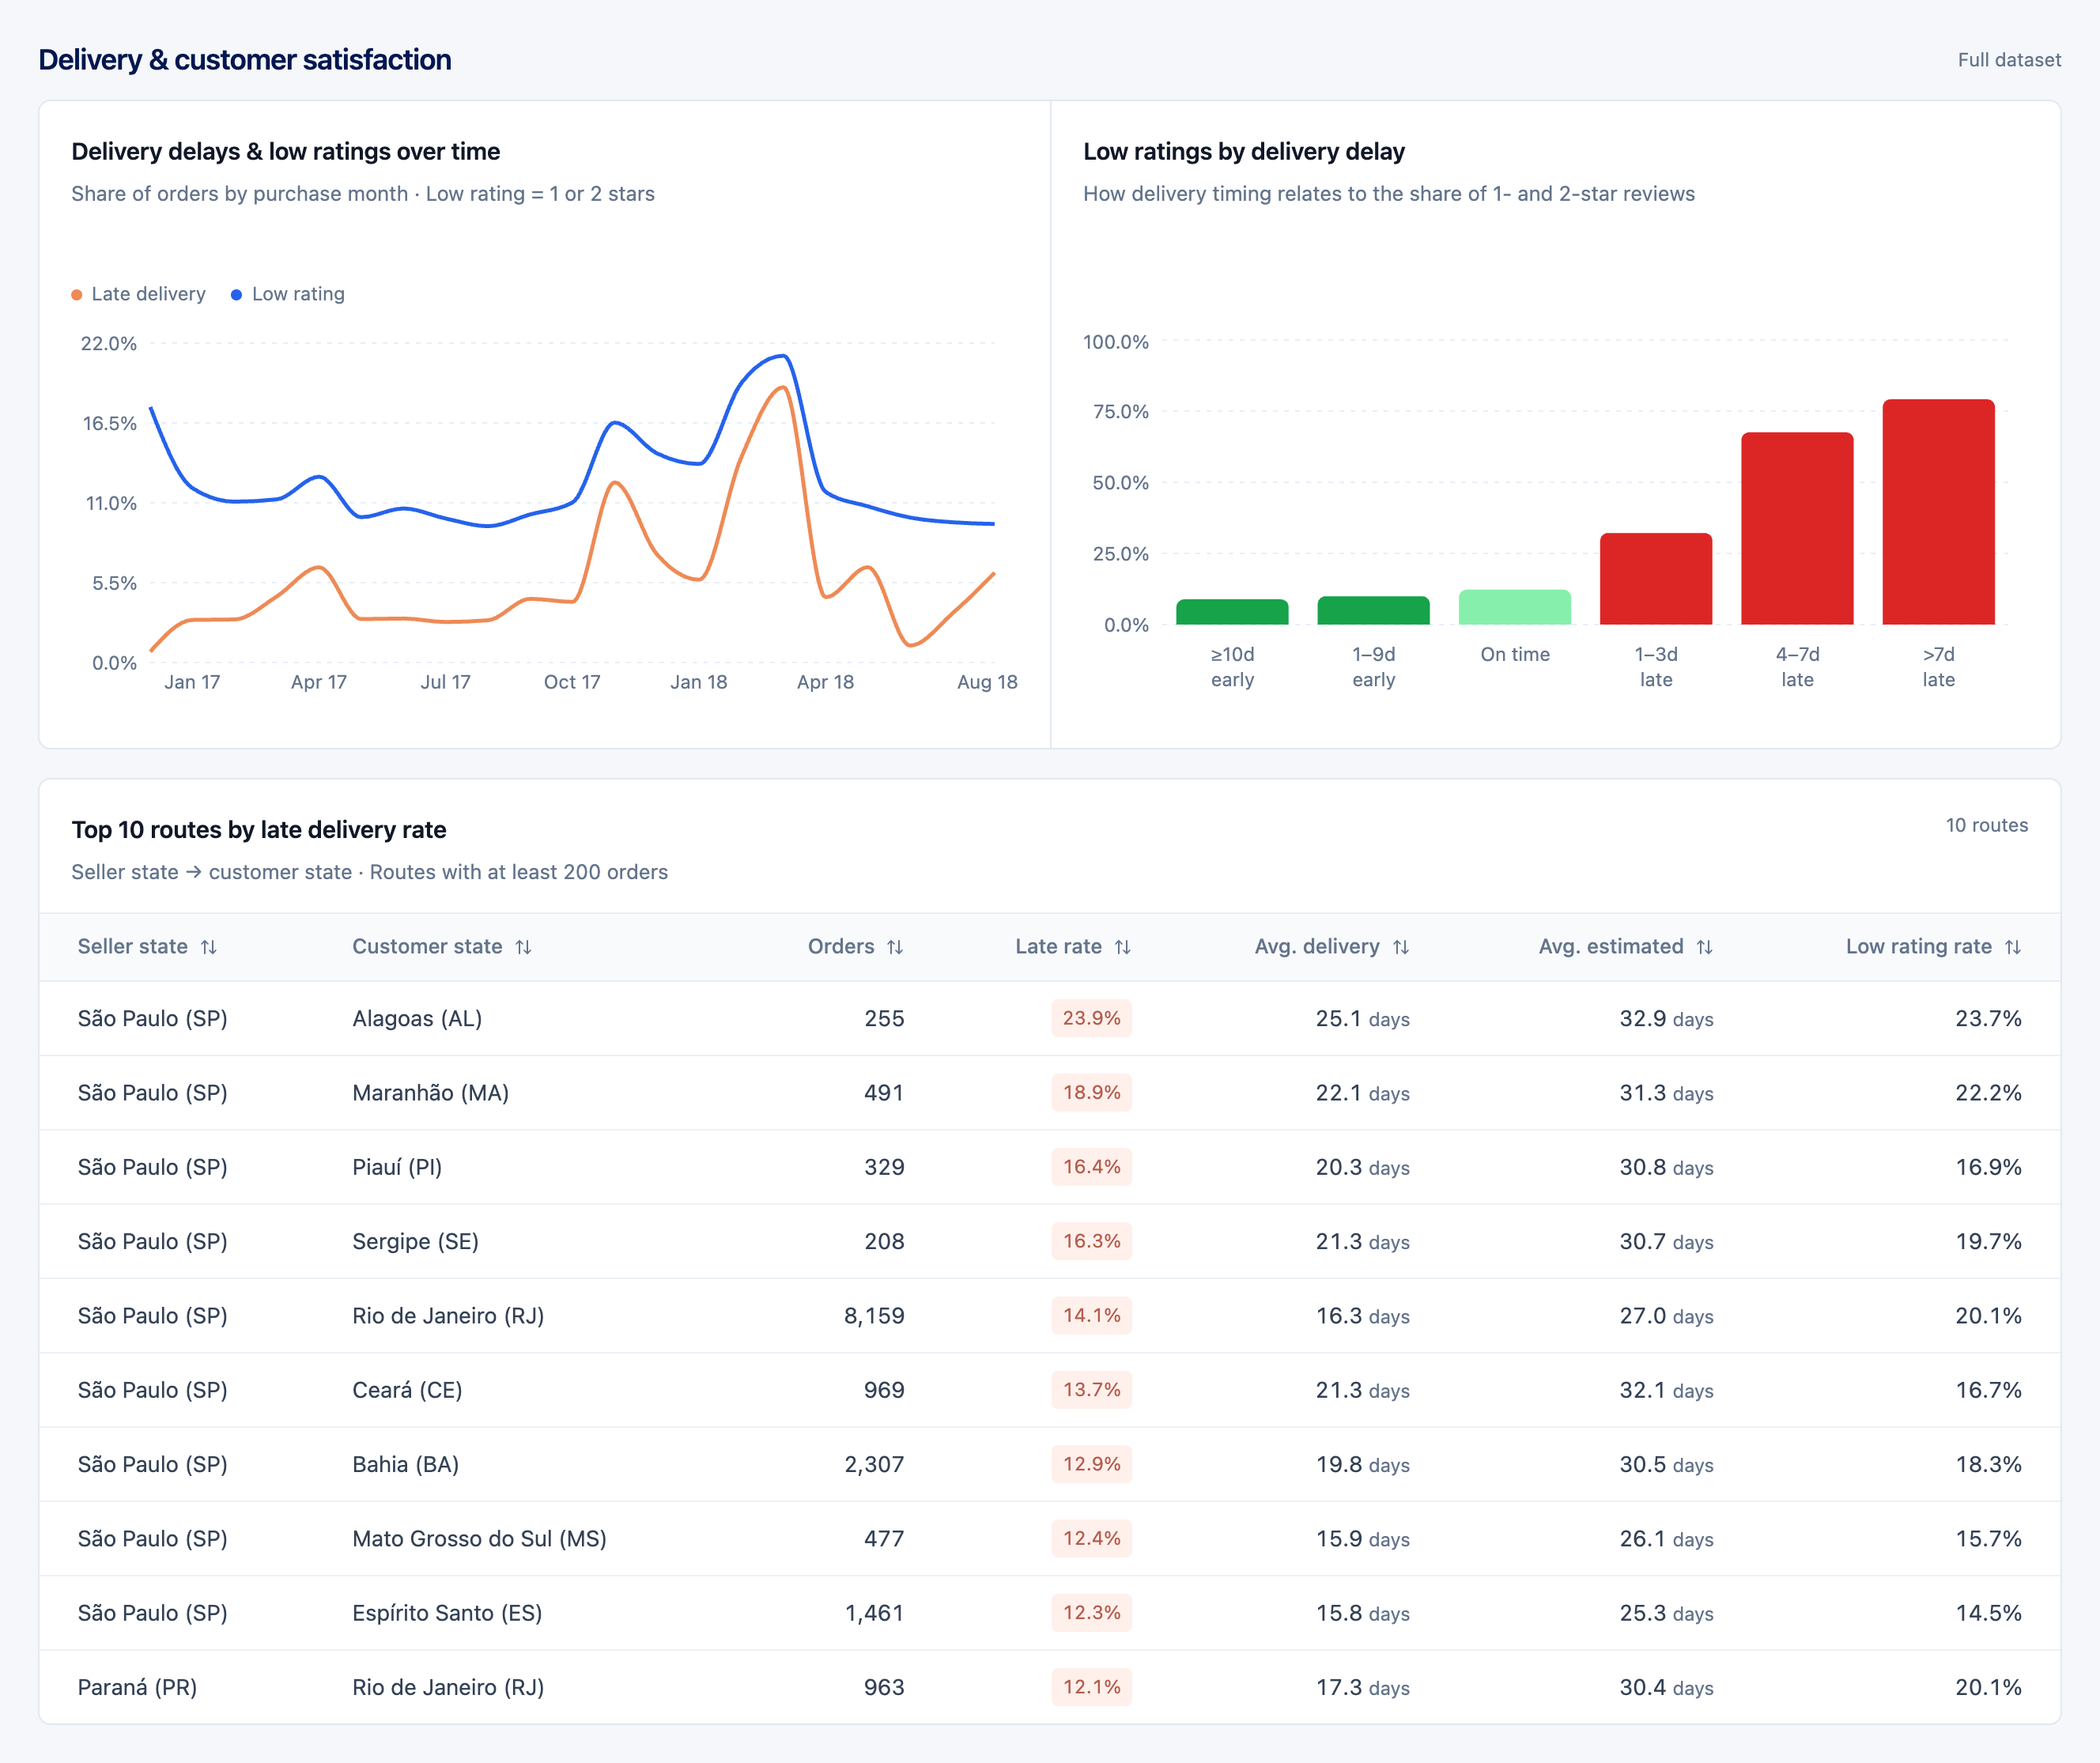
\includegraphics[width=0.75\textwidth]{Picture/ui_manager_delivery.png}
\caption{Manager Dashboard: phần giao hàng và mức độ hài lòng}
\label{fig:ui-delivery}
\end{figure}

\begin{figure}[H]
\centering
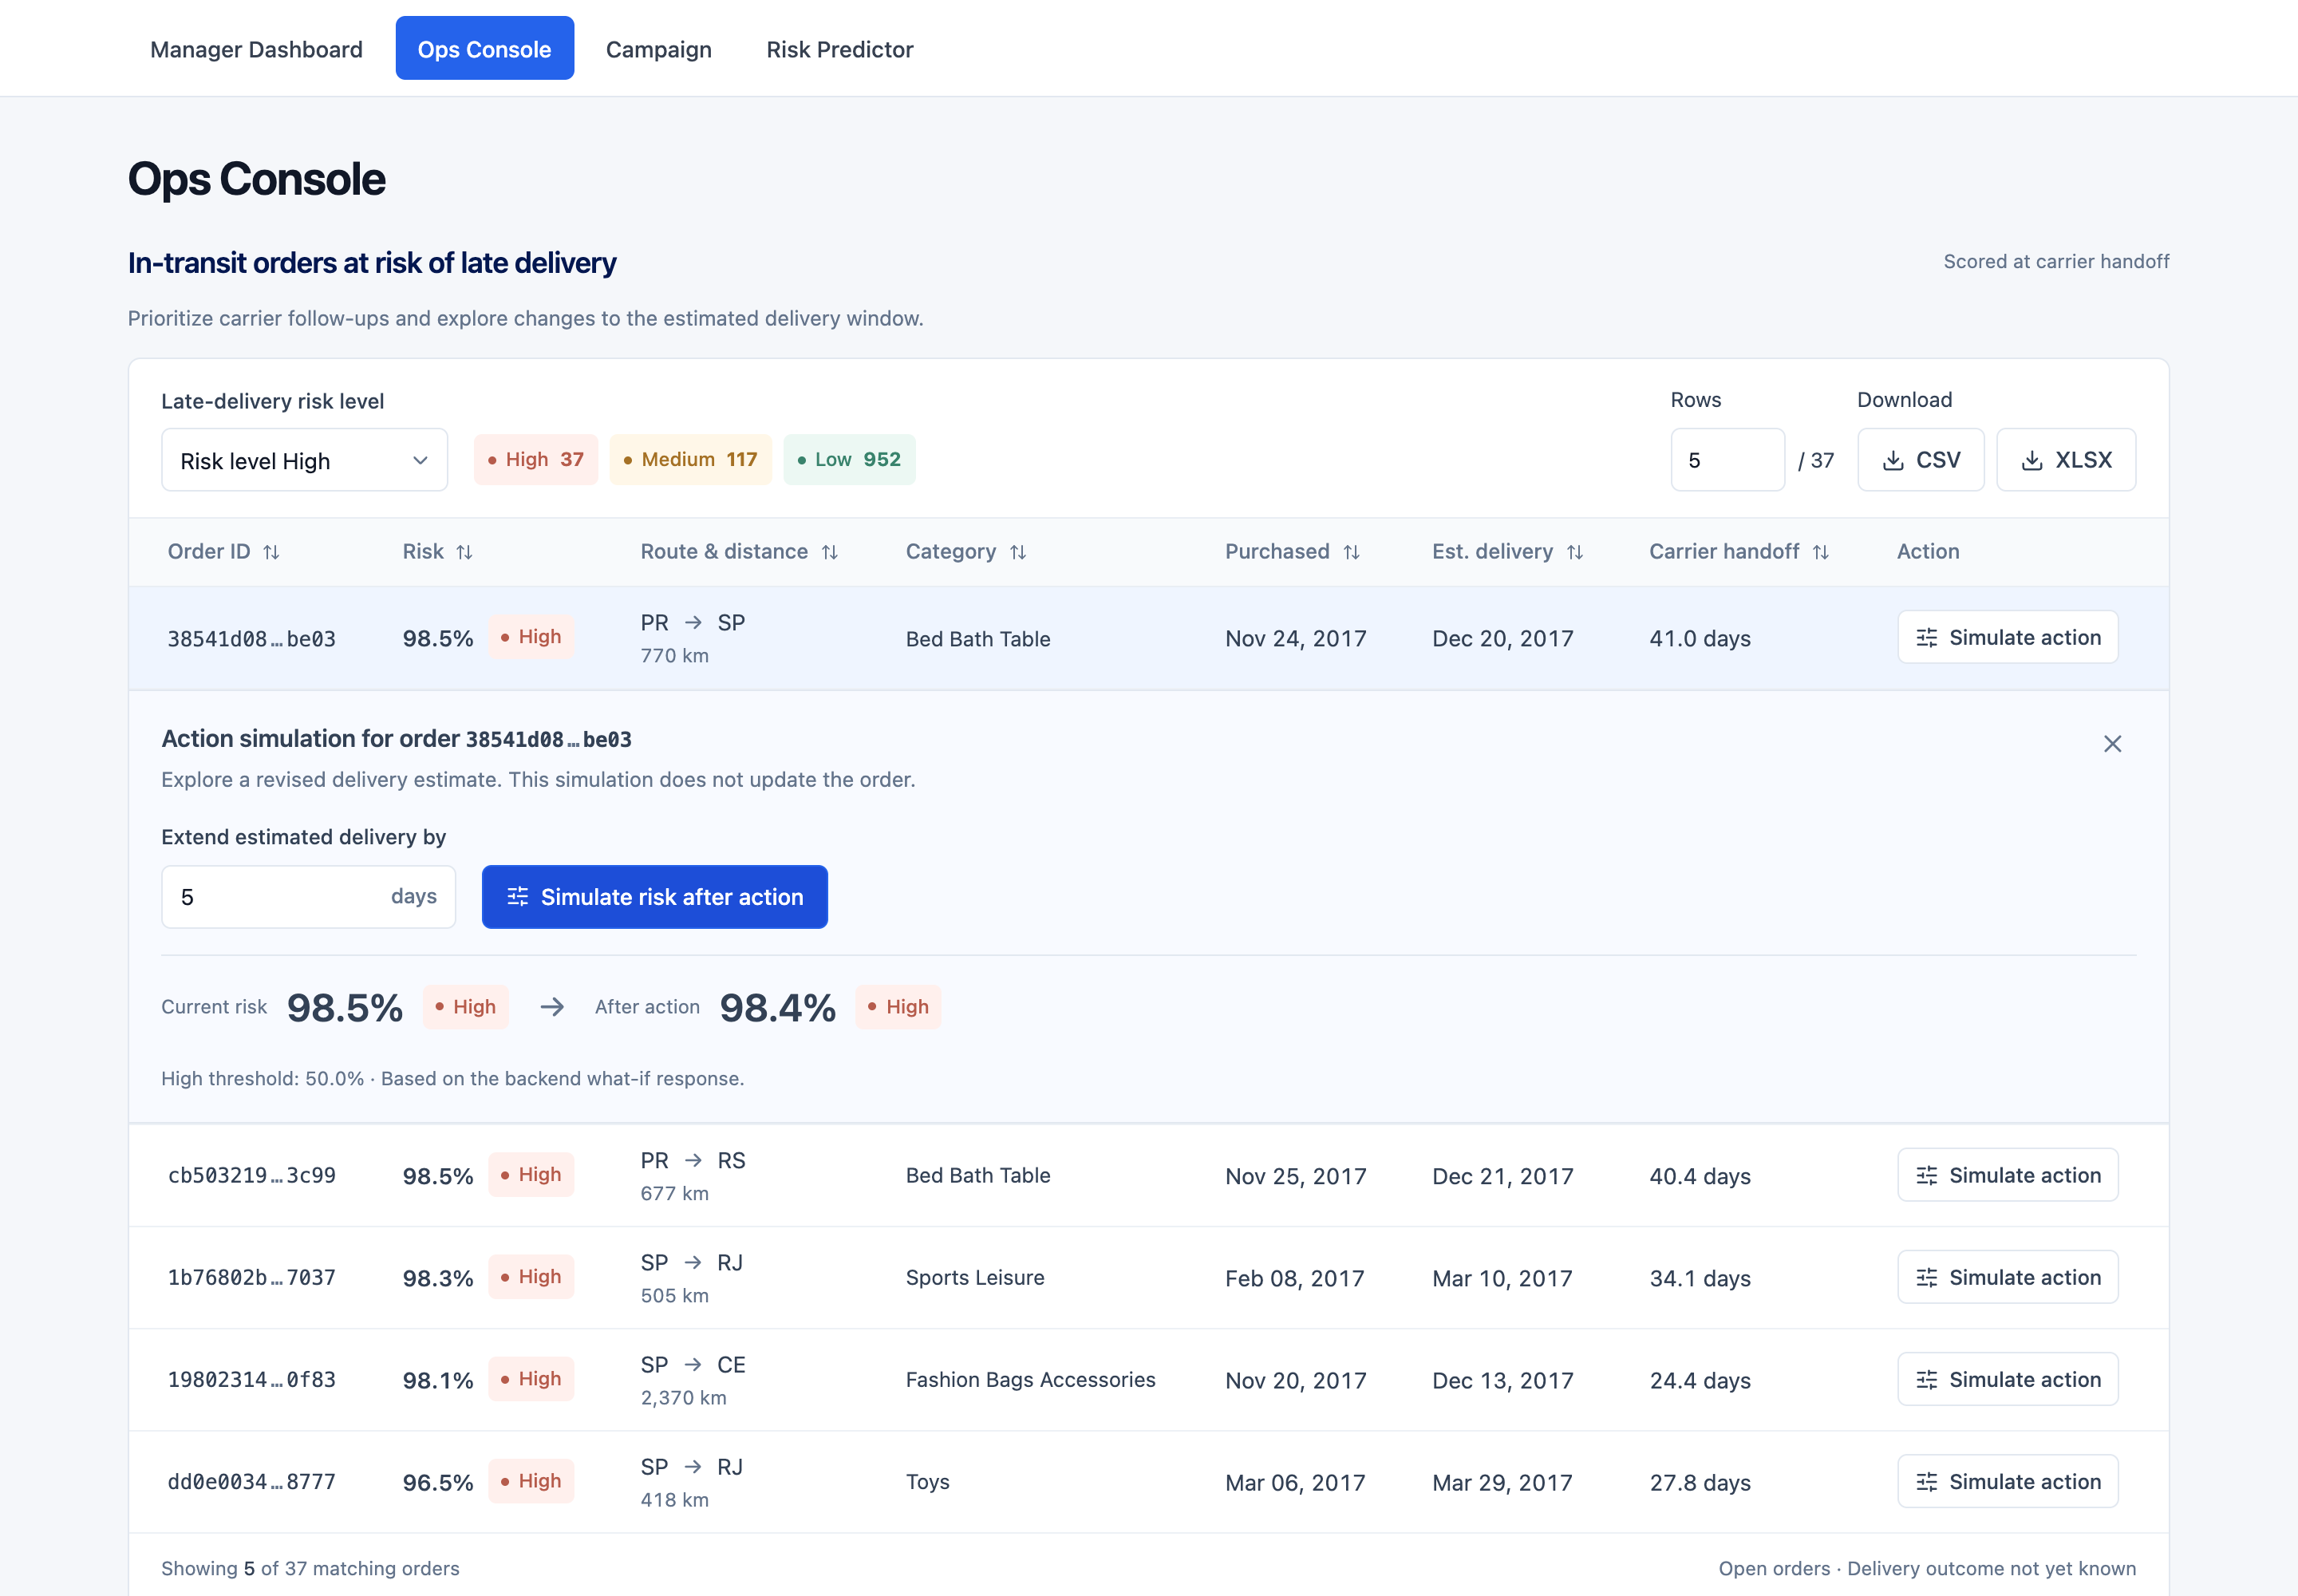
\includegraphics[width=0.75\textwidth]{Picture/ui_ops_late.png}
\caption{Ops Console: danh sách đơn đang vận chuyển có rủi ro giao trễ mức High kèm số đơn theo từng mức, ô chọn số dòng, nút tải CSV/XLSX; khung Action simulation của đơn đầu tiên khi kéo dài ngày hẹn giao 5 ngày (Current risk $\to$ After action)}
\label{fig:ui-ops-late}
\end{figure}

\begin{figure}[H]
\centering
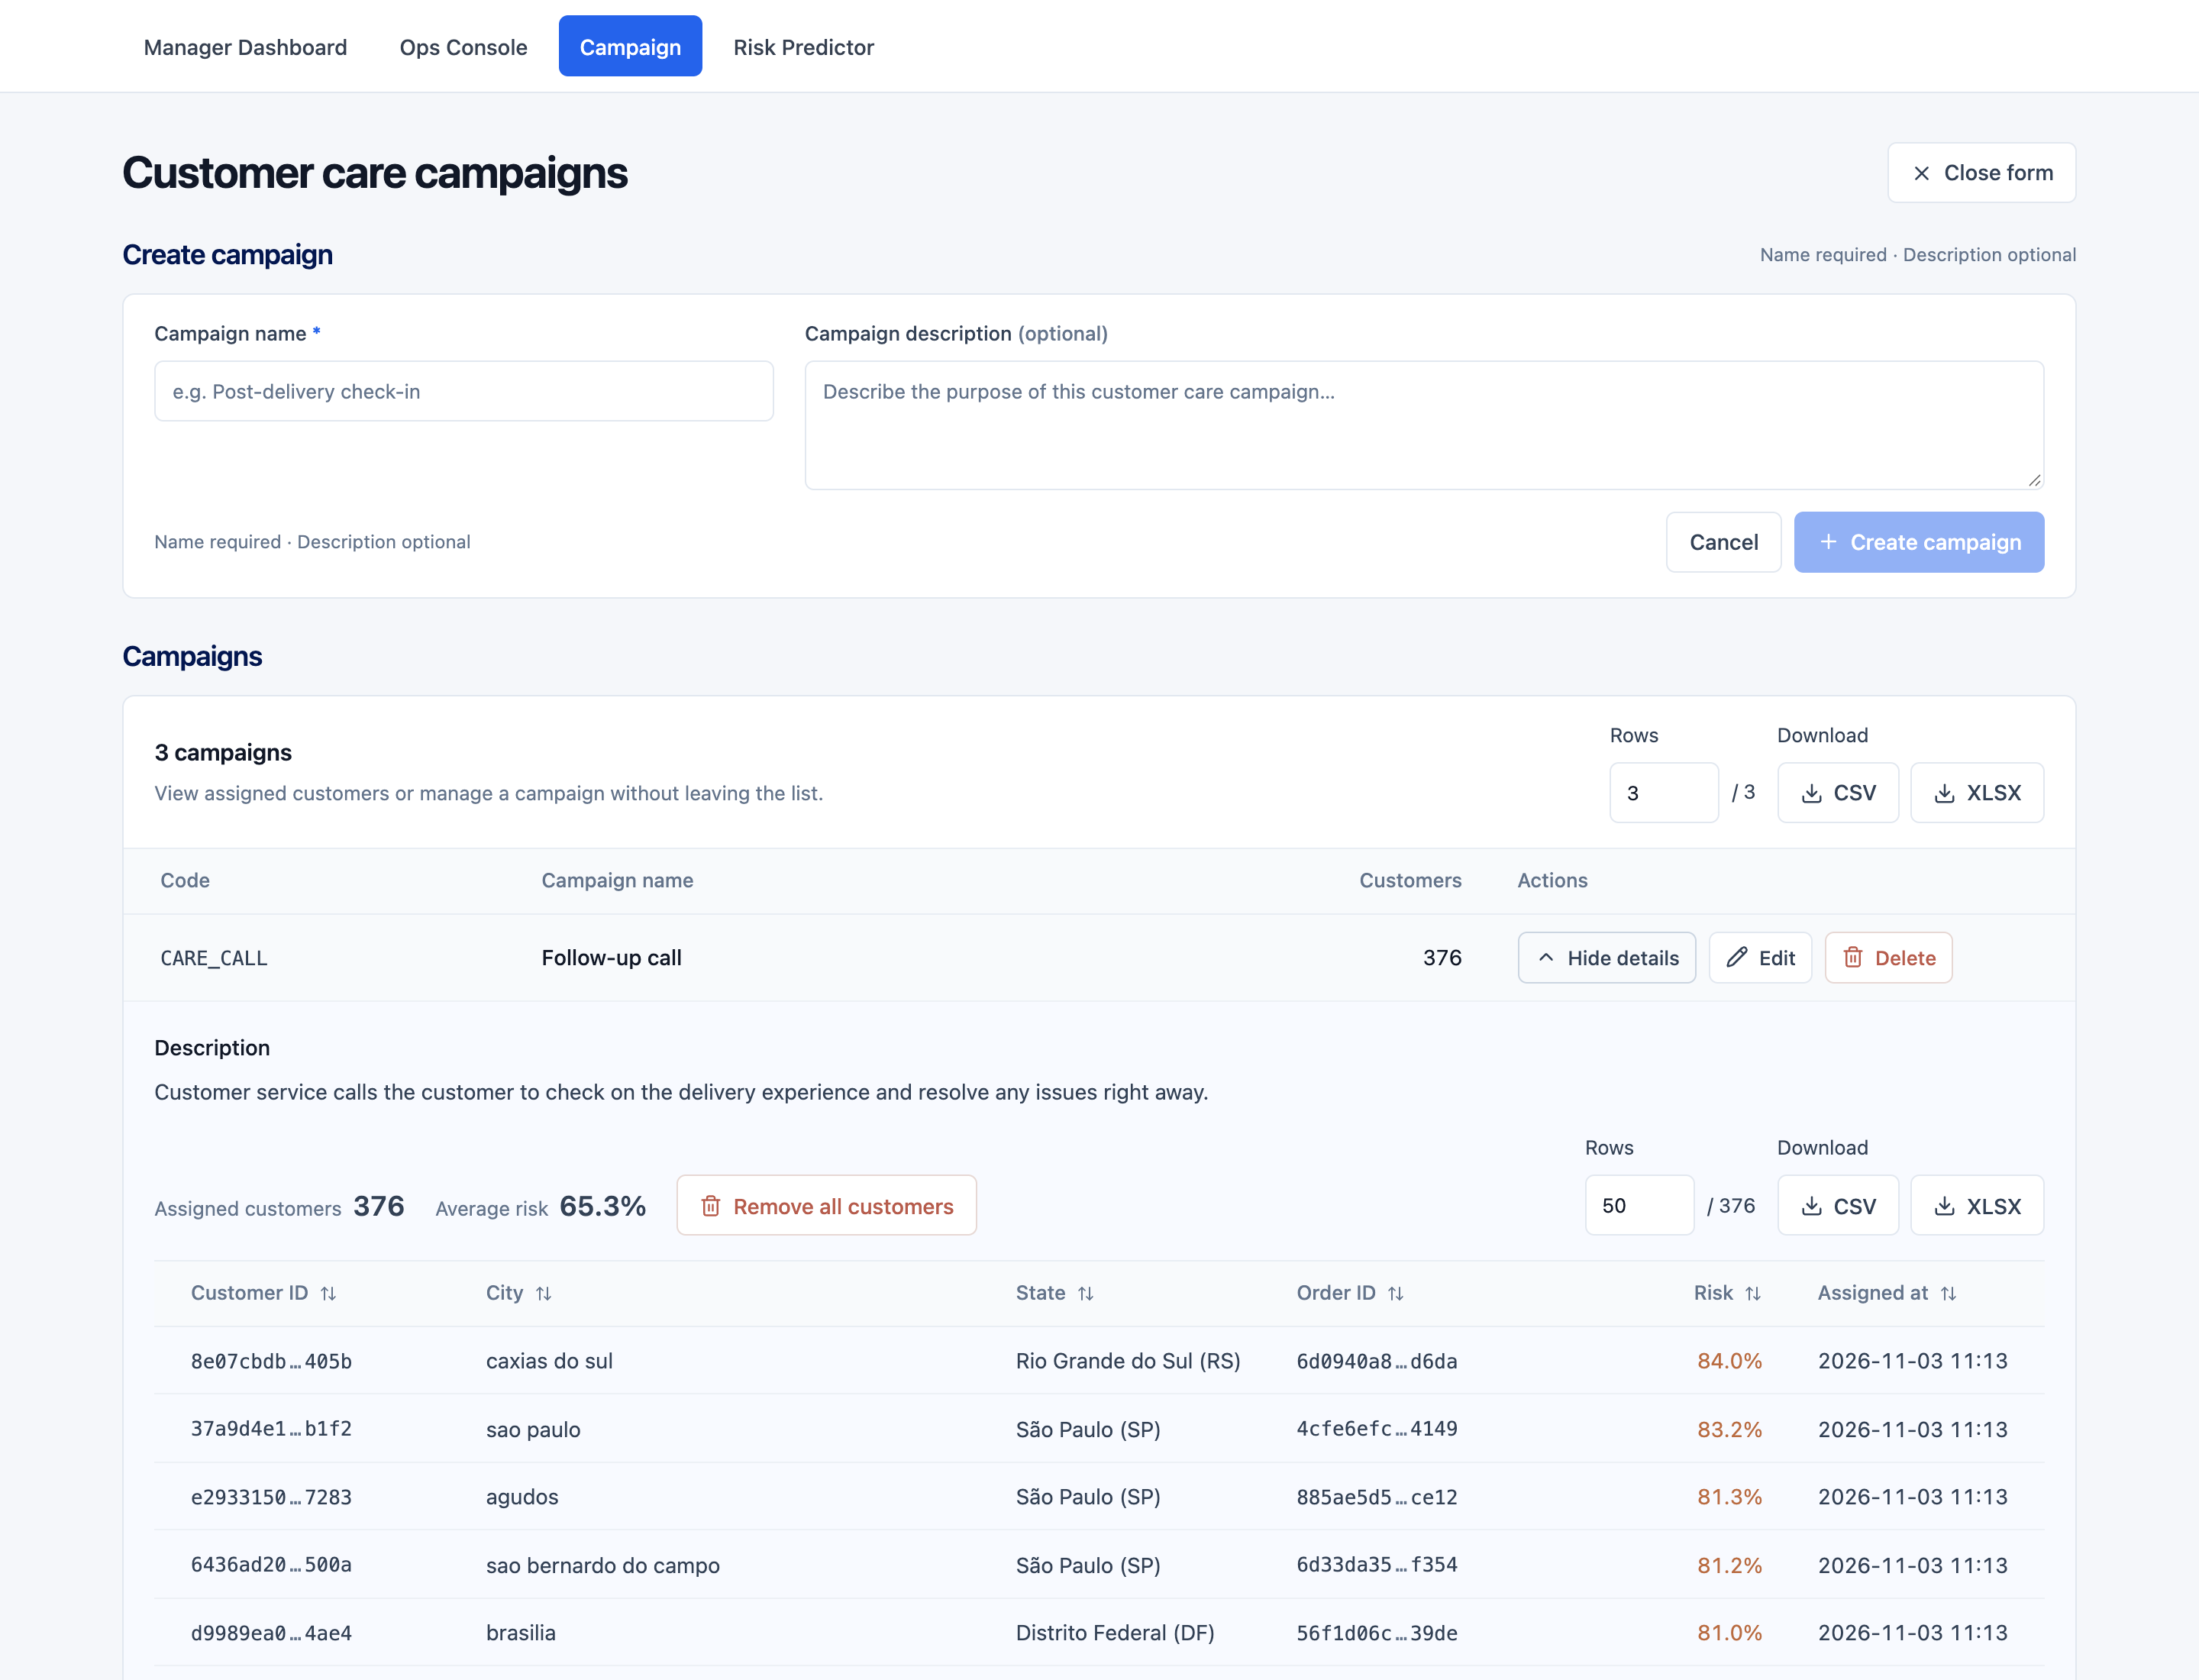
\includegraphics[width=0.75\textwidth]{Picture/ui_campaign.png}
\caption{Màn hình Campaign: danh sách chiến dịch, form thêm mới, phần chi tiết gồm mô tả và khách đã gắn}
\label{fig:ui-campaign}
\end{figure}

\begin{figure}[H]
\centering
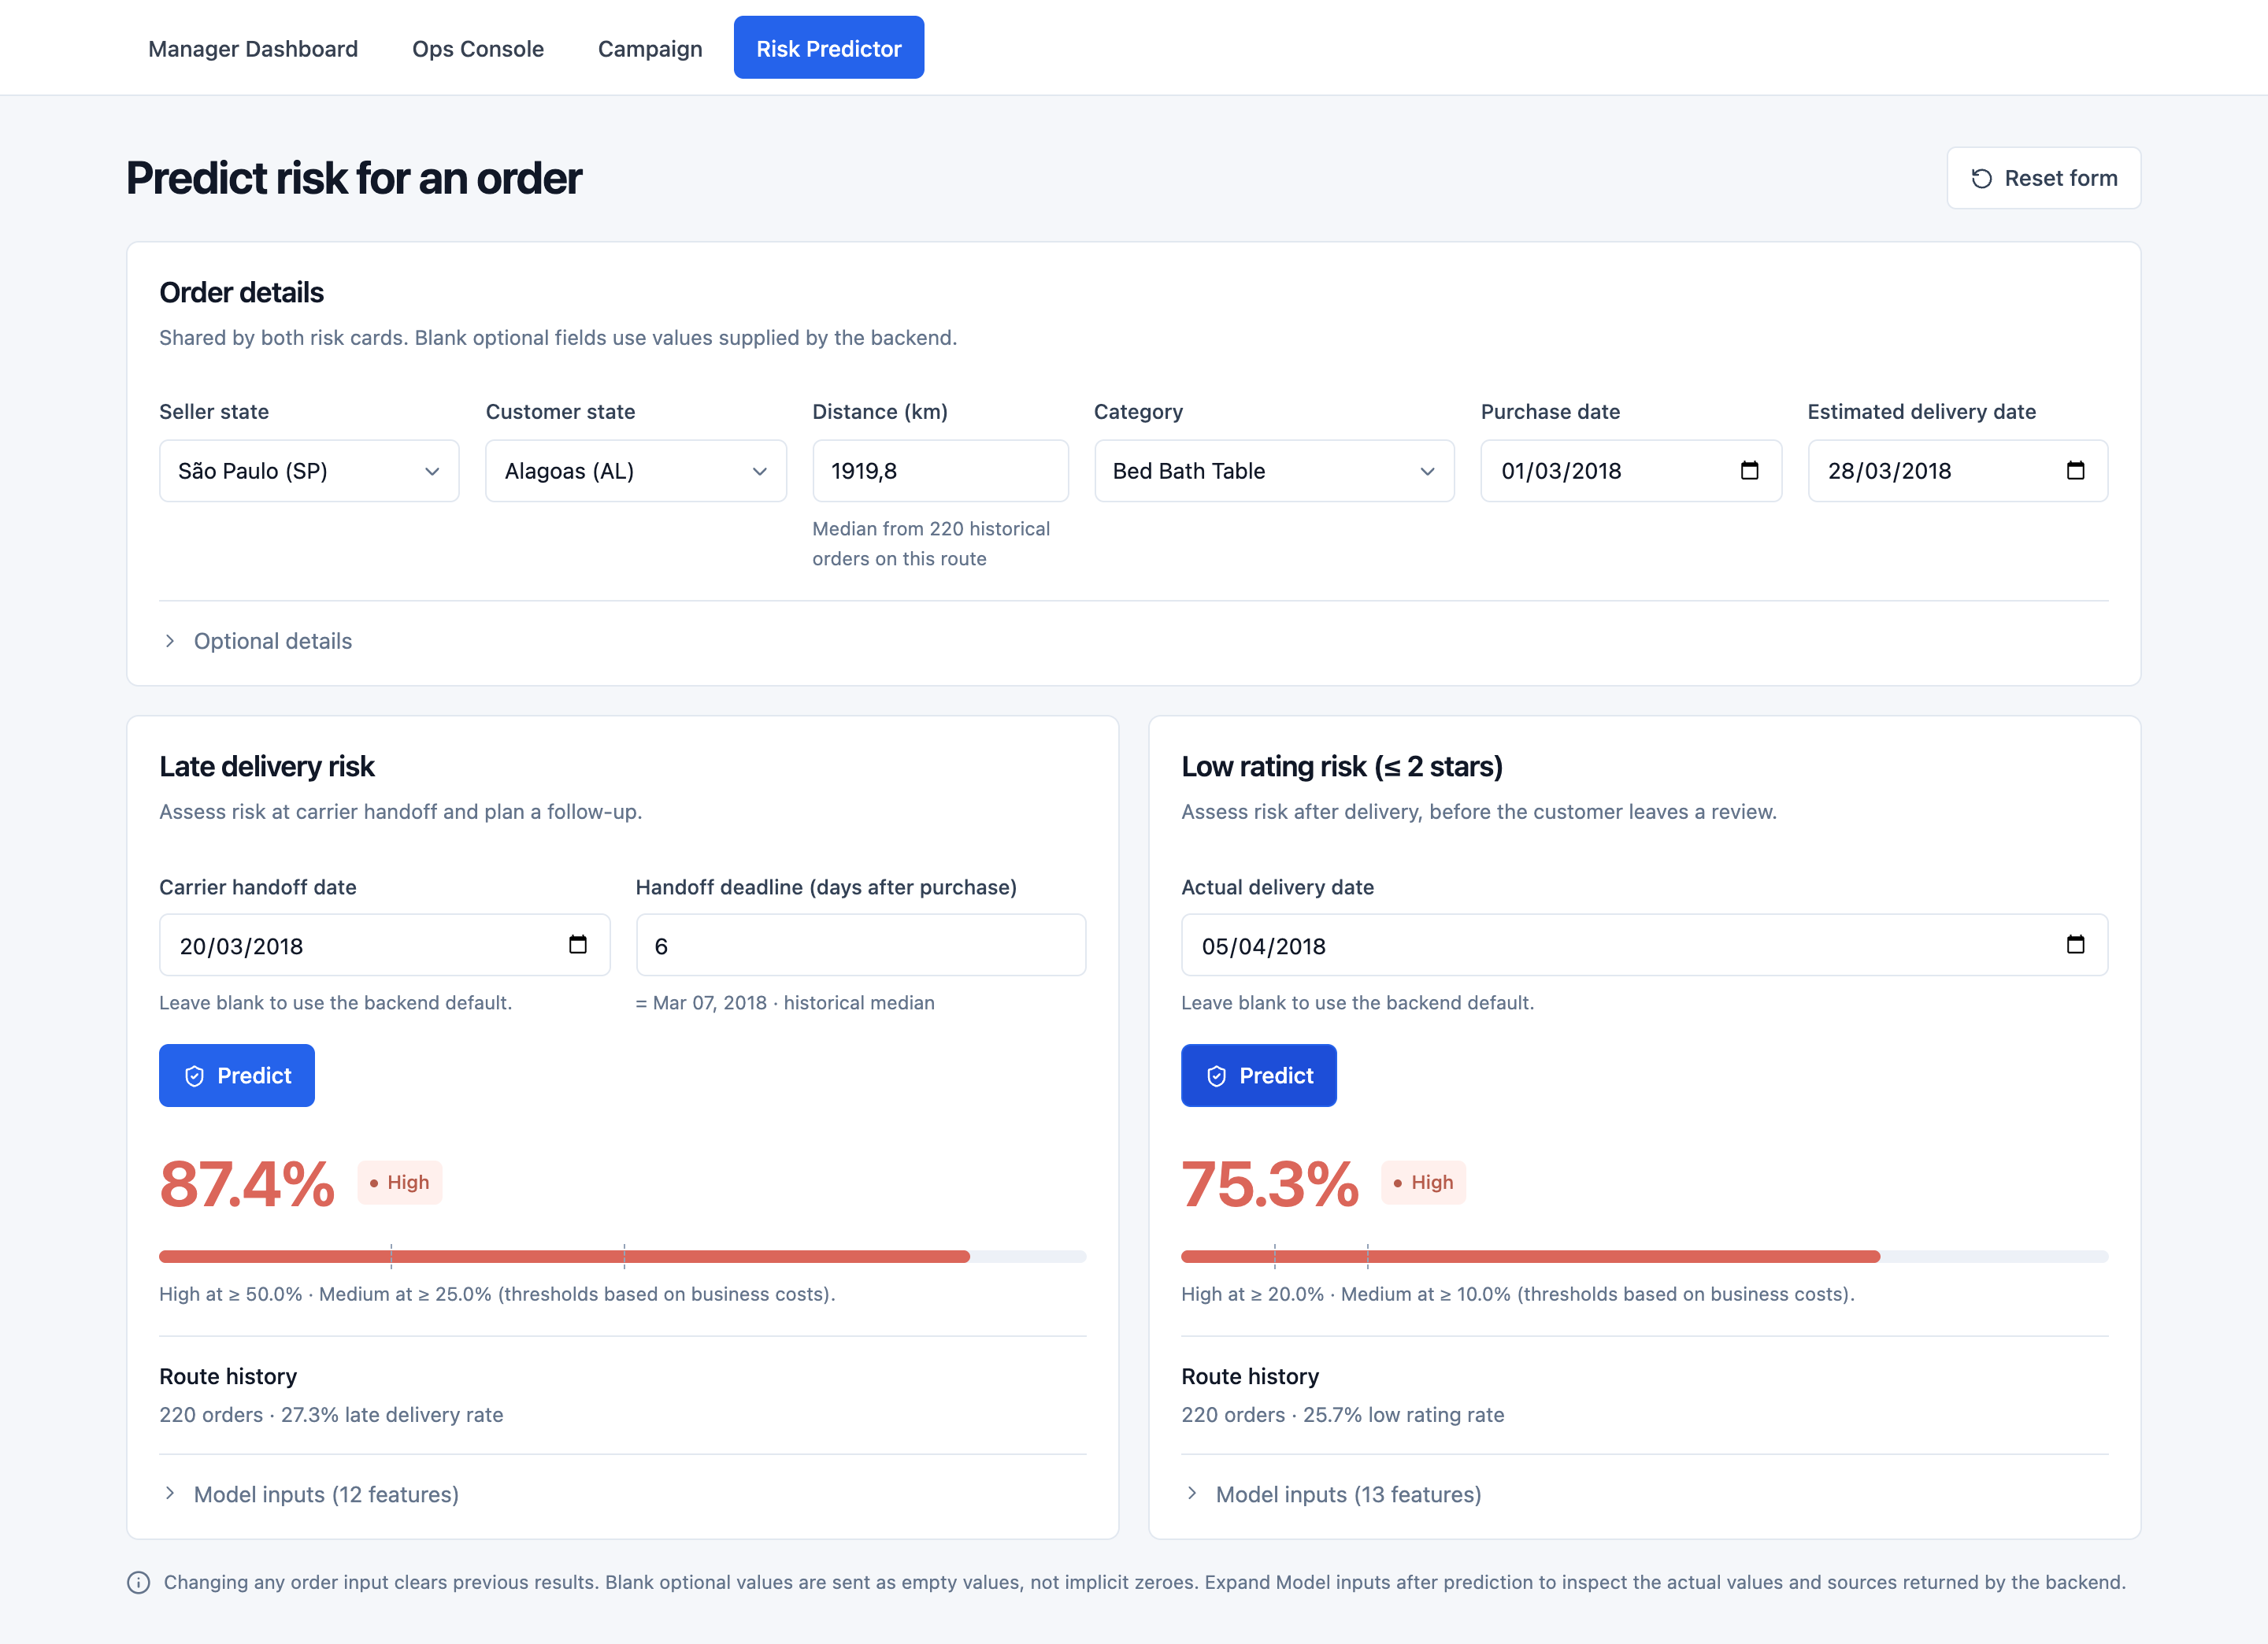
\includegraphics[width=0.75\textwidth]{Picture/ui_predict.png}
\caption{Risk Predictor: đơn giả định tuyến SP $\to$ AL, hẹn giao 27 ngày, người bán bàn giao vào
ngày thứ 19 (rủi ro trễ 87,4\%); nếu giao tới khách trễ 8 ngày thì rủi ro đánh giá thấp 75,3\%}
\label{fig:ui-predict}
\end{figure}
